\section{Prototype Implementation and Evaluation} \label{sec:impl}

We have implemented the sized typing algorithm in a beta version of Coq 8.12~\citep{impl},
which can also be found in the supplementary materials.
Naturally, the full core language of Coq has more features (irrelevant for sized typing) than \lang,
and the implementation has to interact with these as well as other proof assistant features such as elaboration and the vernacular.
Furthermore, many details of the sized typing algorithm are left underspecified.
In this section, we take a take a brief look at these details,
verify the time complexity of the implementation against the theoretical complexities from the previous section,
determine its impact on performance as a whole,
and discuss the practical feasibility of the implementation as well as the problems encountered.

\subsection{Architecture of the Coq Kernel}

The core type checking/inference algorithm is found in Coq's \emph{kernel}.
Before reaching the kernel, terms go through a round of \emph{pretyping}
where existential metavariables (essentially typed holes) are solved for
and the recursive indices of fixpoints are determined.
Size inference is implemented as an augmentation of the existing type checking/inference algorithm,
making use of the recursive indices.

\autoref{fig:kernel} summarizes the relevant file/module structure.
Most of the added code specifically for size inference is in the new \texttt{Sized} and \texttt{Subsizing} modules;
the remaining structure remains the same as that of Coq 8.13's codebase~\citep{coq}.
(\texttt{Subsizing} is only separate from \texttt{Sized} to break circular dependencies: it relies on the global environment, while the environment depends on \texttt{Sized}.)

\begin{figure}
\dirtree{%
.1 coq.
.2 lib.
.3 WeightedDigraph\DTcomment{graph data structure and algorithms for constraints}.
.2 pretyping.
.2 kernel.
.3 Constr\DTcomment{core AST and traversals}.
.3 Environ\DTcomment{environments and lookups}.
.3 Reduction\DTcomment{reduction and convertibility}.
.3 Inductive\DTcomment{functions on (co)fixpoints (guard checking)}.
.3 Typeops\DTcomment{entrypoint to type checker for terms}.
.3 Term\_typing\DTcomment{entrypoint to type checker for declarations}.
.3 Sized\DTcomment{constructs and functions for sized types}.
.3 Subsizing\DTcomment{producing subsizing constraints}.
}
\caption{Selected excerpts of the Coq codebase structure}
\label{fig:kernel}
\end{figure}

The \texttt{Sized} module contains several submodules, four of which are relevant to our performance discussion:
\begin{itemize}
  \item \texttt{State} keeps track of the (position) size variables that have been used;
  \item \texttt{SMap} defines the data structure for and operations on size substitutions;
  \item \texttt{Constraints} defines the data structure for and operations on constraint sets; and
  \item \texttt{RecCheck} implements the \RecCheck and \solve algorithms.
\end{itemize}

Sized typing is implemented as a vernacular flag that can be set and unset, just like guard checking.
By default, the flag is off; the commands
$$\coqinline{Set Sized Typing. Unset Guard Checking.}$$
will enable sized typing only.
If both are set, then guard checking will only occur if sized typing fails.
When sized typing is not set, size annotations are still added, but constraints aren't collected,
meaning that global definitions checked in this state will never be marked as size preserving.

\subsection{Analysis of Performance Degradation}

When compiling parts of the Coq standard library with sized typing on, we noticed some severe performance degradation.
This is bad news if we hope to replace guard checking with sized typing,
or even if we simply wish to use sized typing as the primary method of termination or productivity checking throughout.
In particular, we examine compilation of the \texttt{Coq.MSets.MSetList} library%
\footnote{This file can be found in the artifact at \texttt{coq/theories/MSets/MSetList.v}.},
which is an implementation of finite sets using ordered lists
that contains a fair amount of both fixpoints and proof terms
and that happens to compile successfully with sized typing on.
In this file alone, we find a $5.5\times$ increase in compilation time with \texttt{coqc}.
Other files may have even worse degradation; for an earlier version of the algorithm,
there was a $15\times$ increase in compilation time for \texttt{Coq.setoid\_ring.Field\_theory}%
\footnote{This file can be found in the artifact at \texttt{coq/theories/setoid\_ring/Field\_theory.v}.},
which is about twice as large as \msetlist and contains mostly proofs.
We investigate possible causes of the performance degradation and discuss potential solutions.

\subsubsection{Profiling \texttt{Sized} Functions}

To measure the performance degradation, we compare compiling \msetlist against itself with sized typing on and guard checking off, which we refer to as \msetlistsized.
Both compilations are run five times each.
The compilation times are significantly different ($t = 463.94$, $p \ll 0.001$),
with \msetlist's compilation time at $15.122 \pm 0.073$ seconds and \msetlistsized's at $82.660 \pm 0.286$ seconds.

\begin{table}
\centering
\begin{tabular}{| l | r | r | r | r |}
\hline
\textbf{Function(s)} & \textbf{Unsized time (s)} & \textbf{Sized time (s)} & \textbf{$t$} & \textbf{Sized time \%} \\
\hline
\textbf{\solve}               & $ 0.029 \pm 0.002$ & $ 62.397 \pm 0.414$ &  337 &  74.6  \\
\textbf{\RecCheck}            & $ 0.000 \pm 0.000$ & $  2.203 \pm 0.023$ &  219 &   2.63  \\
\textbf{\texttt{Constraints}} & $ 0.186 \pm 0.005$ & $  2.899 \pm 0.028$ &  217 &   3.46 \\
\textbf{\texttt{SMap}}        & $ 0.011 \pm 0.001$ & $  0.281 \pm 0.003$ &  215 &   0.34 \\
\textbf{\texttt{State}}       & $ 0.047 \pm 0.002$ & $  0.104 \pm 0.002$ &   55 &   0.12 \\
\textbf{\texttt{foldmap}}     & $ 0.163 \pm 0.004$ & $  0.266 \pm 0.004$ &   46 &   0.32 \\
\hline
\textbf{Total of above}       & $ 0.436 \pm 0.014$ & $ 68.150 \pm 0.474$ &      &  81.5  \\
\textbf{Total compilation}    & $15.122 \pm 0.073$ & $ 83.660 \pm 0.286$ &      & 100    \\
\hline
\end{tabular}
\caption{Relevant function runtimes when compiling \msetlist vs. \msetlistsized}
\label{table:timing}
\end{table}

To identify the source of the slowdown and test our hypothesis that the majority of it
is intrinsically due to size inference,
we first profile the performance of functions relevant to the \texttt{Sized} module during the compilation.
We divide these functions into five groups: the \solve and \RecCheck functions,
the \texttt{foldmap}%
\footnote{This is the \texttt{foldmap\_annots} function in \texttt{coq/kernel/Constr.ml}.}
function common to all operations manipulating size annotations on the AST (such as applying size substitutions),
the functions in \texttt{State}, the functions in \texttt{SMap}, and the functions in \texttt{Constraints}.
\autoref{table:timing} summarizes the results, as well as the relative time spent in the functions in \msetlistsized.
The differences in execution times of the functions in each group are all statistically significant ($p \ll 0.001$ for all of the $t$-statistics).
% meaning that the differences between the sized and unsized times are statistically significant.

$77.2\%$ of the total compilation time in \msetlistsized is taken up by \solve and \RecCheck.
Other \texttt{Sized}-related overhead is smaller, although not insignificant,
especially \texttt{Constraint} operations, which form a proportion slightly larger than that of \RecCheck.
We conjecture that some of this other overhead can be reduced with more clever implementations.
For instance, instead of explicitly performing size substitutions, the sizes can be looked up as needed;
or instead of explicitly passing around a size state, we could use a state monad or a mutable global state;
or constraints could be stored in a data structure incrementally checked for negative cycles,
similar to the current implementation of universe level constraints.
We therefore focus our attention on \solve and \RecCheck, where performance degradation may not be limited to mere implementational details.

% TODO: Don't flow this manually...
\begin{figure}
\begin{subfigure}{0.475\textwidth}
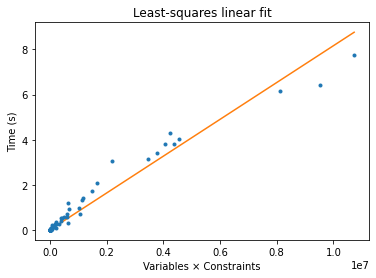
\includegraphics[width=0.9\textwidth]{images/least-squares-solve.png}
\caption{\solve execution time vs. $\norm{V}\norm{C}$ \\ (blue dots), linear model (orange line)}
\label{fig:stats:linregress-solve}
\end{subfigure}
\hfill
\begin{subfigure}{0.475\textwidth}
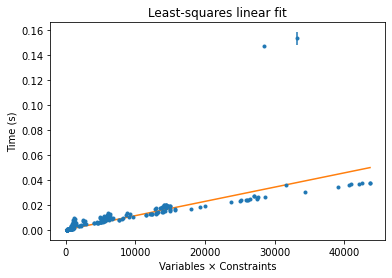
\includegraphics[width=0.9\textwidth]{images/least-squares-RecCheck.png}
\caption{\RecCheck execution time vs. $\norm{V}\norm{C}$ \\ (blue dots), linear model (orange line)}
\label{fig:stats:linregress-reccheck}
\end{subfigure}
\\[3ex]
\begin{subfigure}{0.475\textwidth}
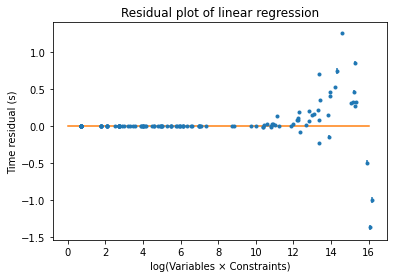
\includegraphics[width=0.9\textwidth]{images/residuals-solve.png}
\caption{\solve model residuals plot (log scale)}
\label{fig:stats:residuals-solve}
\end{subfigure}
\hfill
\begin{subfigure}{0.475\textwidth}
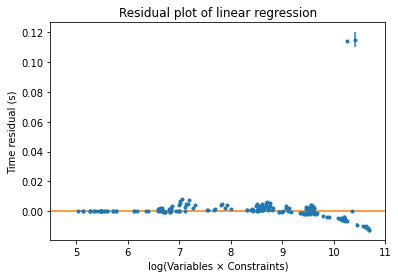
\includegraphics[width=0.9\textwidth]{images/residuals-RecCheck.png}
\caption{\RecCheck model residuals plot (log scale)}
\label{fig:stats:residuals-reccheck}
\end{subfigure}
\\[3ex]
\begin{subfigure}{0.475\textwidth}
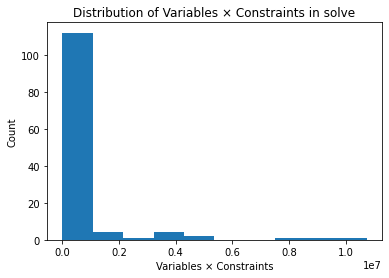
\includegraphics[width=0.9\textwidth]{images/distribution-solve.png}
\caption{$\norm{V}\norm{C}$ distribution in \solve, 10 bins}
\label{fig:stats:distr-solve}
\end{subfigure}
\hfill
\begin{subfigure}{0.475\textwidth}
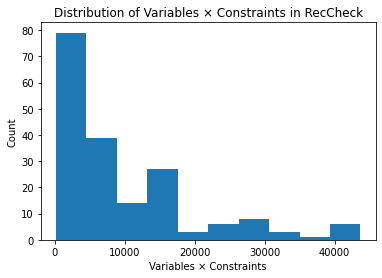
\includegraphics[width=0.9\textwidth]{images/distribution-RecCheck.png}
\caption{$\norm{V}\norm{C}$ distribution in \RecCheck, 10 bins}
\label{fig:stats:distr-reccheck}
\end{subfigure}
\\[2ex]
\caption{Execution vs. $\norm{V}\norm{C}$, residuals, $\norm{V}\norm{C}$ distributions for \solve and \RecCheck}
\label{fig:stats}
\end{figure}

\begin{figure}
\begin{minted}{coq}
Unset Guard Checking.
Set Sized Typing.
Time Definition nats1  := (nat, nat, nat, nat, nat, nat, nat, nat).
Time Definition nats2  := (nats1, nats1, nats1, nats1).
Time Definition nats3  := (nats2, nats2, nats2, nats2).
Time Definition nats4  := (nats3, nats3, nats3, nats3).
Time Definition nats5  := (nats4, nats4, nats4, nats4).
Time Definition nats6  := (nats5, nats5, nats5, nats5).
\end{minted}
\caption{Coq definitions with an explosion in size variables and elapsed time}
\label{fig:nats}
\end{figure}

\subsubsection{Time Complexity of \titlesolve and \titleRecCheck}

As shown in \autoref{sec:algorithm}, given a constraint graph from constraint graph $C$ with size variables $V$,
the time complexities of \solve and \RecCheck are $O(\norm{V}\norm{C})$.
Indeed, in \autoref{fig:stats:linregress-solve},
plotting the mean execution times of each of the 155 calls to \solve against $\norm{V}\norm{C}$ for that call (shown as blue dots),
we see a strong positive correlation ($r = 0.983$).
Doing the same for the 186 calls to \RecCheck in \autoref{fig:stats:linregress-reccheck},
we have a weaker positive correlation ($r = 0.698$),
likely due to the two visible outliers.
(Without the outliers, we have $r = 0.831$.)

To verify that the execution times are dominated by linear relationships to $\norm{V}\norm{C}$,
we fit the data to linear models using least-square regressions (shown as orange lines),
and examine the residuals plots in \autoref{fig:stats:residuals-solve} and \autoref{fig:stats:residuals-reccheck}
for \solve and \RecCheck, respectively.
(Note the logarithmic horizontal scale used for clarity, as there are more calls with fewer variables and constraints).

For \solve, the model appears to be a good fit at first,
but residuals increase in magnitude as $\norm{V}\norm{C}$ increases,
indicating some additional behaviour unexplained by the model.
Similarly, for \RecCheck, the model also appears to be a good fit at first,
but then follow a downward curving pattern,
also indicating additional behaviour unexplained by the model (such as the two outliers).

Although there might be additional smaller factors influencing the time complexities of \solve and \RecCheck beyond the number of variables and constraints,
we can at least reasonably conclude that execution time increases with $\norm{V}\norm{C}$.
Since this time complexity is intrinsic to the algorithms and is not due to mere implementational details,
and more than three-fourths of the total compilation time is due to $\solve$ and $\RecCheck$,
the majority of the slowdown is therefore intrinsic and unavoidable.

\subsubsection{An Explosion of Size Variables}

As $\solve$ and $\RecCheck$ contribute so much to the compilation time
and their complexities depend on $\norm{V}\norm{C}$,
there must be a significant number of calls involving large numbers of variables and constraints.
Indeed, \autoref{fig:stats:distr-solve} and \autoref{fig:stats:distr-reccheck}
show that despite most calls during compilation of \msetlist involving small values of $\norm{V}\norm{C}$,
the number of calls with large values of $\norm{V}\norm{C}$ is not trivial.

Of course, the presence of large numbers of variables and constraints of only \msetlist with sized typing
doesn't tell us whether this is a common property of Coq files on average,
but the fact that this occurs in the standard library indicates that it is absolutely possible
for an explosion in size variables and constraints to be a significant barrier to the adoption of sized typing for general-purpose use.
In fact, this behaviour is easily reproducible with the artificial but comparatively small and simple example in \autoref{fig:nats}.
\autoref{table:nats-stats} lists the number of size variables present in the types and bodies of these definitions,
along with the elapsed type checking time reported by Coq.

\begin{table}
\centering
\begin{tabular}{| l | r | r | r | r |}
\hline
\textbf{Definition} & \textbf{$\norm{V}$ (body)} & \textbf{$\norm{V}$ (type)} & \textbf{Time (s)} \\
\hline
\coqinline{nats1}  &  14    & 7    &  0.004 \\
\coqinline{nats2}  &  62    & 31   &  0.020 \\
\coqinline{nats3}  &  254   & 127  &  0.177 \\
\coqinline{nats4}  &  1022  & 511  &  2.299 \\
\coqinline{nats5}  &  4094  & 2047 & 35.385 \\
\coqinline{nats6}  &  16382 & 8191 & $>120$ \\
\hline
\end{tabular}
\caption{Size variables and time elapsed for definitions in \autoref{fig:nats}}
\label{table:nats-stats}
\end{table}

There are two things we can do to reduce the execution time of \solve and \RecCheck:
eliminate constraints when possible, or reduce the number of size variables in definitions.
One way to accomplish the first option would be to turn on sized typing only for certain definitions,
in particular the ones involving \cofixpoints where they will be most useful.
Then for all other definitions, since no constraints are collected,
calls to \solve will be trivial regardless of how many size variables they contain.

However, a \cofixpoint might require that some non-\corecursive definition with many size variables be size preserving,
which means that that definition also needs to be checked with sized typing on,
or the \cofixpoint itself may have a large number of size variables.
Furthermore, there's no clear indication of which definitions might have a large number of size variables and which don't,
leaving it up to a lot of guesswork and experimentation.
Using sized typing as a targeted tool for particular programs is not viable
if we cannot directly tell \emph{which} particular programs will benefit the most
in terms of tradeoffs between non-structural \corecursion and performance.

The second option to reduce the number of size variables can be done by allowing manual annotation of \coinductive types with the infinite size,
reducing the number of free size variables that need to be substituted for
and that propagate throughout subsequent definitions.
For example, the tuple types in \autoref{fig:nats} can have infinite size annotations
without affecting the sizes of the \coqinline{nat} arguments.
In other words, we allow size annotations in the surface language that users write,
which would no longer be plain CIC;
as this solution deviates from the philosophy of being wholly backward compatible,
it is beyond the scope of this paper.

\subsection{Inferring Recursive Indices}\label{sec:impl:recind}

As previously mentioned, users aren't obligated to indicate which fixpoint argument is the one on which we recur,
and its position index is inferred during pretyping in the kernel.
In Coq, for a mutual fixpoint, this is done by trying the guard predicate on every combination of indices%
\footnote{This is the \texttt{search\_guard} function in \texttt{coq/kernel/Pretyping.ml}.}.
This is possible because the guard predicate is a syntactic check, requiring nothing but the elaborated fixpoint term.

Unfortunately, we run into problems when attempting to apply the same strategy to inferring recursive indices through sized typing alone.
Because termination checking is inextricably tied to type checking,
the entire fixpoint needs to be type checked to verify whether the current set of indices is correct,
and this type checking in the kernel can fail if the fixpoint still contains unsolved metavariables.
Furthermore, because we only have access to the bare environments (\ie with no sizes inferred),
local definitions in scope at the fixpoint may not yet known to be size preserving,
thus causing the check to fail.
As an example, in the following Coq term, \coqinline{id} has no size annotations and is therefore treated as \emph{not} size preserving,
even though it ought to be, which causes the recursive call on the smaller argument wrapped in \coqinline{id} to not pass type checking.
%
\begin{minted}{coq}
let id (x : nat) := x in
  fix f (n : nat) :=
    match n with
    | O => O
    | S k => f (id k)
    end
\end{minted}
%
This suggests that size inference should be done during the pretyping phase:
size inference could be viewed as part of the elaboration step from the surface CIC to the core \lang.
This, too, is beyond the scope of this paper, especially as there is no past work on the interaction between size inference and elaboration to build on.
